\documentclass[10pt]{extarticle}

\usepackage[utf8]{inputenc}              % Tipos de caracteres
\usepackage[portuguese]{babel}           % Português
\usepackage[a4paper,portrait]{geometry}  % Tipo de papel
\usepackage{color}                       % Para tratamento da cor
\usepackage{graphicx}                    % Para a imagem
\DeclareGraphicsExtensions{.jpg,.png}
\usepackage{amsmath}                     % Para as matematiquices
\usepackage{amssymb}
\usepackage{array}
\usepackage{gensymb}                     % Grau
\usepackage{multicol}
\setlength{\columnsep}{1cm}
\usepackage{geometry}					% Margens
%\usepackage{xfrac}
\usepackage{colortbl}

\usepackage{multirow}

\addtolength{\topmargin}{-20mm}
\addtolength{\textheight}{50mm}
\addtolength{\oddsidemargin}{-15mm}
\addtolength{\textwidth}{32mm}

\renewenvironment{abstract}
 {\small
  \begin{center}
  \bfseries \abstractname\vspace{-.5em}\vspace{0pt}
  \end{center}
  \list{}{
    \setlength{\leftmargin}{0cm}%
    \setlength{\rightmargin}{\leftmargin}%
  }%
  \item\relax}
 {\endlist}
 
\renewcommand{\abstractname}{Resumo}

\delimitershortfall-1sp
\newcommand\abs[1]{\left|#1\right|}
\newcommand{\PR}[1]{\ensuremath{\left[#1\right]}}
\newcommand{\PC}[1]{\ensuremath{\left(#1\right)}}
\newcommand{\chav}[1]{\ensuremath{\left\{#1\right\}}}

\newcolumntype{x}[1]{>{\centering\hspace{0pt}}p{#1}}

\begin{document}

\title {\bf \huge T0 - Caracterização de uma Célula Fotovoltaica}
\author
{{\small Grupo III - João Ferreira (78179) Henrique Rodrigues (78632) Rodrigo C. Carvalho (78646) Cristina Melício (78947)} \\
{\small MEFT - 2ºAno, 2º Semestre - Laboratório de Complementos de Eletromagnetismo e Termodinâmica}}
\date{{\small Sexta-Feira, 27 de Fevereiro de 2014}}
\maketitle

\begin{multicols}{2}

\section{Protocolo Experimental}

\subsection{Preparação da experiência}

\begin{enumerate}
\item Efectue a montagem do circuito representado na figura 1:

\hspace{-1.6cm}
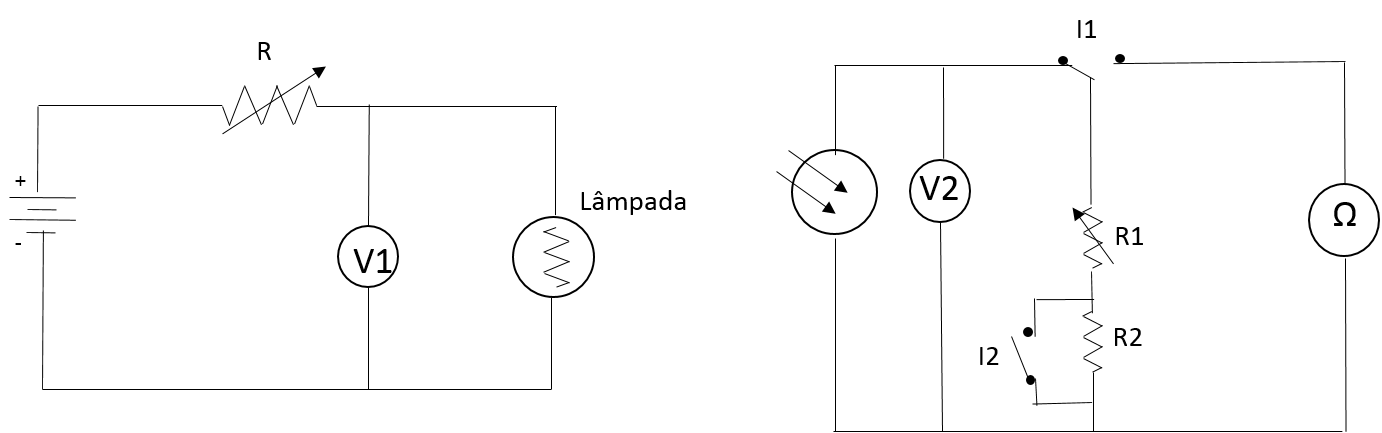
\includegraphics[width=260pt]{circuito}

\begin{center}
\par\noindent {\scriptsize (Figura 1: Esquema da montagem)}
\end{center}

\item Confirme o alinhamento da lâmpada e a célula fotovoltaica na escala, a uma distância de $25cm$.

\item Ligue a fonte de tensão, verificando através do voltímetro 1 que o valor da tensão não ultrapassa os 12V por forma a não danificar o filamento da lâmpada. 

\end{enumerate}

\subsection{Característica Eléctrica da Célula Fotovoltaica}

\begin{enumerate}

\item  Coloque a célula a um ângulo de $0^\circ$. Utilizando o interruptor 1 da caixa de resistências, ligue alternadamente o circuito que permite medir o valor indicado no ohmímetro e aquele que permite medir o valor indicado no voltímetro. Varie o valor da resistência da caixa de resistências entre $0\Omega$ e $3200\Omega$ (indicado no ohmímetro) e com o interruptor 1 na outra posição meça para cada valor a tensão nos terminais na célula fotovoltaica (indicado no voltímetro).

\par\noindent \textbf{Nota 1:} Para alcançar as resistências mais altas poderá ter de mudar a posição do interruptor 2 de modo a incluir a resistência $R2$.

\item Determine a corrente através da lei de Ohm: 

\begin{equation}
U=RI \Leftrightarrow I=\frac{U}{R}
\end{equation}

\item Determine a característica da célula fotovoltaica (relação tensão-corrente) através dos dados obtidos.

\item Repita o procedimento para um conjunto de ângulos entre $0^\circ$ e $90^\circ$ tendo o cuidado de manter a face da célula sobre a qual incide a luz proveniente da lâmpada virada para cima, de modo a evitar reflexão luminosa.

\item Represente no mesmo gráfico as curvas características.

\end{enumerate}

\subsection{Determinação da resistência de carga ótima}

\item Obtenha a potência a partir da resistência e da tensão a partir da seguinte relação:

\begin{equation} \label{eq2}
P=UI=\frac{U^2}{R}
\end{equation}

\item Para cada ângulo considerado anteriormente, encontre o máximo de potência, cujo maximizante corresponde, por definição, à resistência de carga óptima.

\subsection{Determinação de relações de linearidade}

\begin{enumerate}

\item Sabendo que a intensidade que atinge a célula fotovoltaica depende do ângulo $\alpha$ entre a normal da superfície da célula e a luz incidente da seguinte forma:

\begin{equation}
I\propto\cos{\alpha}
\end{equation}

\par\noindent considere o nível de iluminação em percentagem.

\item A partir das curvas característica obtidas, procederá agora à determinação de eventuais relações de linearidade entre a intensidade luminosa e as seguintes grandezas:
\begin{enumerate}
\item Corrente com tensão fixa $U_0$.
\item Tensão com corrente fixa $I_0$.
\item Potência com resistência fixa $R_0$.
\item Valor da resistência de carga ótima.
\item Valor da potência máxima.
\end{enumerate}
\end{enumerate}

\par Para analisar as três primeiras relações, estude a intersecção dos gráficos obtidos, respetivamente, com uma recta do tipo $y=U_0$, com uma recta do tipo $x=I_0$ e com uma recta de declive $R_0$.
\par\noindent \textbf{Nota 2:} Caso os valores que tenha não sejam conclusivos, retire novamente dados para uma nova amplitude.

\subsection{Determinação da lei da variação da potência fornecida à carga pela célula fotovoltaica com a distância desta à fonte luminosa}

\begin{enumerate}
\item Fixe um valor de resistência.
\item Varie a distância entre a lâmpada e a célula fotovoltaica, medindo para cada valor de distância o valor da Tensão através do voltímetro.
\item Efectue o procedimento acima descrito para diversos ângulos. 
\item Obtenha os valores da potência através da equação \eqref{eq2} e determine a lei da variação da potência fornecida à carga pela célula fotovoltaica com a distância desta à fonte luminosa.
\end{enumerate}

%\section{Introdução}

%\par 

%\begin{equation} \label{eq:1}
%\gamma = \frac{1}{\sqrt{1-\frac{v^2}{c^2}}}
%\end{equation}

%\begin{center}
%\par\noindent {\scriptsize (onde ...)}
%\end{center}

%\section{Procedimento Experimental}

%\begin{center}
%\includegraphics[width=240pt]{ftg9}
%\end{center}

%\begin{center}
%\begin{tabular}{ x{0.4cm} x{1.1cm} x{1.1cm} x{1.1cm} x{1.1cm} }
%i & $p_x$ & $\varepsilon_{p_x}$ & $p_y$ & $\varepsilon_{p_y}$ \tabularnewline 
% & {\scriptsize $(MeV/c)$} & {\scriptsize $(MeV/c)$} & {\scriptsize $(MeV/c)$} & {\scriptsize $(MeV/c)$} \tabularnewline 
%\hline \hline
%\multicolumn{5}{x{6.5cm}}{Método 1} \tabularnewline
%\hline \hline
%1      & -2033 & -   & 0    & -  \tabularnewline
%3      & 766   & 68  & 383  & 31 \tabularnewline
%4      & 291   & 34  & -430 & 45 \tabularnewline
%$\sum$ & -976  & 102 & -47  & 75 \tabularnewline
%\hline \hline
%\multicolumn{5}{x{6.5cm}}{Método 2} \tabularnewline
%\hline \hline
%1      & -2033 & -  & 0    & -  \tabularnewline
%3      & 775   & 68 & 395  & 40 \tabularnewline
%4      & 306   & 30 & -437 & 42 \tabularnewline
%$\sum$ & -952  & 98 & -43  & 81 \tabularnewline
%\end{tabular}
%\end{center}

%\begin{center}
%\par\noindent {\scriptsize (Tabela 3: Momentos lineares e seu balanço, referentes à colisão da fotografia 9)}
%\end{center}

%\section{Análise de Resultados e Conclusões}

%\par 

%\vfill

%\pagebreak

%\section{Anexos}

%\subsection*{\normalsize Material}

%\begin{itemize}
%\item D
%\end{itemize}

%\subsection*{\normalsize Tabelas Completas de Resultados}

%\begin{center}
%\begin{tabular}{ x{2cm} x{2cm} x{2cm} }
%Partícula & $m$ {\scriptsize $(MeV/c^2)$} & $q/q_{p^+}$
% \tabularnewline
%\hline \hline
%$p^+$   & $938$ & 1 \tabularnewline
%$n^0$   & $939$ & 0 \tabularnewline
%$\pi^0$ & $135$ & 0 \tabularnewline
%$\pi^+$ & $140$ & 1 \tabularnewline
%\end{tabular}
%\end{center}

%\begin{center}
%\par\noindent {\scriptsize (Tabela 1A: Massa e carga das partículas analisadas)}
%\end{center}

%\subsection*{\normalsize Fórmulas de Erro}

%\begin{equation}
%\varepsilon_{p_{col}}=\frac{E_i}{c^2p_{col}}\varepsilon_l
%\end{equation}

\end{multicols}

\end{document}